
\documentclass[5p]{elsarticle}
\usepackage{natbib}
\usepackage{url}
\usepackage{subcaption}
\begin{document}
\title{Creating updated, scientifically-calibrated mosaics for the RC3 Catalogue}
\maketitle 

\section{Introduction}
Astronomical catalogs such as the famous Messier Catalog and New General Catalog (NGC) has its historical usage in helping  astronomers who are studying objects that shares some common property. This was particularly important in the days when all-sky information was not available, so data was taken by pointing the telescope at some particular location.  
%before the era of large surveys like SDSS, DSS and 2MASS that scanned large portions of the sky  instead of target-based imaging.
Wide sky surveys such as the Sloan Digital Sky Survey(SDSS), Digitized Sky Survey (DSS), and Two Micron Sky Survey (2MASS) not only provide improved astrometry for finding these objects, but also photometric ,(other info?) on detected sources, such as those generated through SDSS's $\texttt{photo}$ pipeline (CITE).
%Astronomical catalog usage in the age of sky surveys for studies 
%RC3 Completeness versus accuracy
With large sky surveys such as the SDSS, the job of target-based imaging is alot easier since the position values of objects of interest are readily accesible via NED/ SIMBAD. The role of the astronomical catalogue has evolved into sample for statistical studies for some particular type of object (QSO, pulsars,LRG...etc) or cosmology studies.
%can also be used for data mining and machine learning training sets (??)
\\
\indent 
The Third Reference Catalog of Bright Galaxies (RC3) compiled by \citet{rc3}, contains a  complete listing of 23,022 galaxies with $D\_25$ apparent major isophotal diameter  greater than 1 arcminute and with a total B-band magnitude greater than 15.5 nanomaggies.
The RC3 Catalog is an update of the original Reference Catalog of Bright Galaxies. It is 
<TALK ABOUT DATA, ViZier. HOW OFTEN UPDATED..etc?> 
\\
\indent
There has been existing literature on making mosaics for RC3 galaxies using data from the Sloan Digital Sky Survey(SDSS). Hogg and Blanton made g,r,i colored images of selected RC3 galaxies by using data from the SDSS DR6.\footnote{\url{http://cosmo.nyu.edu/hogg/rc3/}} The EFIGI catalog (\citet{efigi}), dedicated to studying morphology of galaxies, also  obtained a subset of 4458 RC3 FITS and color images using SDSS DR4 data and discarded artifacted or missing data via visual inspection. We perform the mosaicing procedures on the whole RC3 catalog using an automated positional update algorithm on the most recent SDSS DR10 imaging data. In addition, we designed a mosaicing pipeline that creates scientifically-calibrated mosaics, color-band images, as well as a set of updated positions, which can be easily adapted for existing surveys such as Two Micron All Sky Survey  (2MASS),The Palomar Digital Sky Survey (DPOSS), or future imaging data release from  Dark Energy Survey (DES) and Large Synoptic Survey Telescope (LSST) for larger sky coverage and multiband images.
%tools such as Aladin, NED/SIMBAD, VizieR. 
\section{Data}
	\section{The RC3 Catalog}
	% Stuff from Corwin's email (maybe use a section to discuss disadvantages of RC3 data)
 %what the RC3 doesn't have is the faint stuff that some astronomers are more interested in 
 %it ismissing all the big, nearby dwarf galaxies and "star streams" that SDSS has been finding -- to say nothing of the other faint Local Group galaxies thatpeople are turning up -- and it relies on the Johnson-Cousins system for its basic photometric calibration (diameters as well as magnitudes and colors).

	Since the RC3 catalog is a reasonably complete representation of large, bright nearby galaxies in the extragalactic sky, its 
%The value of the RC3 catalog 
value is still evident in its usage in literature. Selected galaxies or complete subsets are used in astrophysical studies of  quasars and X-ray sources% (\citett{xray})
 or  galaxy morphology and properties(CITE).  The RC3 catalog is also statistical studies  for cosmology purposes Cross correlated also used in  Updated Catalog, such as the New York University-Value Added Galaxy Catalog (NYU-VAGC)

	\subsection{Positional Inaccuracy in RC3 Catalog}
Original Reference Catalogue of Bright Galaxies (CITE)
	uniform update ``collected from 150 different sources" ,each telescsope has different acccuratcy precision..etc
	The principle motivation behind the automation algorithm is to resolve the problem of centering galaxies and finding RC3 galaxy in a given field of view. Initially, using the standard mosaicking steps in Montage, we obtained many images with  off-centered or missing galaxies due to the inherent inaccuracy of the positions in the catalog. 
	%This was not due to wrong coordinate frame conversion from B2000 to J2000 since the effects should be negligible in terms of centering a galaxy but due to the inherent inaccuracy of the positions given by the RC3 Catalog
There is an non-uniform update of the catalog over the years (-----) after the catalog was publish, more accurate position was collected from whatever sources/data they had access to.
The B2000 coordinates (FK4 frame) in the RC3 catalog are denoted with two different levels of accuracy: HH MM SS.s, DD MM SS for the positions that has been updated  (with accuracy of about 5-8 arcsec) and  HH MM.m, DD MM for galaxies whose positional accuracy remain  1-2 arcminutes in the original catalog.  In the latest version of the catalog (\citet{rc31991}), there remains 5492 RC3 galaxies that fall in the latter group.
\subsection{Data}
(INSERT FIGURE WITH ONE OBJECT MOSAICED FROM ALL DIFFERENT SURVEEYS, SIDE BY SIDE )
	\subsubsection{SDSS}
	SDSS is a optical 
	2.5m telescope at the Apache Point Observatory in New Mexico. We use the imaging data from Data release 10 which is part of the SDSS-III. SDSS-III is dedicated to studying galaxy clustering by looking at signatures of Baryon Acoustic Oscillation,structure and history of the galaxy , and the population of expolanets. Feeding the SDSS data into the mosaicing pipeline has several advantages over data from other surveys, 
1) It is  one of the newest all-sky survey so has improved instrumentation and telescope compared to DPOSS. 
2)On a related note, the resolution of SDSS is better than 2MASS and DPOSS.  2MASS has a ``Tile" size, each Tile, so each pixel represents ----degree, whihc is much larger than  SDSS's pixel size of ----. 
	
(TALK ABOUT HOW SDSS IMAGING DATA IS PROCESSED; SEE PHOTOLITE PAPER LUTPON) 	 The SDSS data is pass through ----pipline, deblending, source , 
	SKyServer provide many info
	

	\subsection{2MASS}
	 The Two Micron All Sky Survey (2MASS; \citet{2mass}) is a infared survey in the J(1.25 $\mu$m), H(1.67 $\mu$m), and K(2.17 $\mu$m) bands. Data taken from two 1.3m telescope  covered 99.998\% of the sky where each ``survey tile" is 6 degree long by 8.5 arcminute strip. Since the RC3 catalog contains large nearby galaxies, we narrowed down our imaging data search to  2MASS's  Extended Source Catalogs which contained only 1.6 million identified object instead of Point Source Catalog which contained 471 million identified sources. (Does 2MASS have more advantage in seeeing ``cooler" object that give off thermal radiation? ) The motivation in using 2MASS data is its large all-sky cover, however since each ``survey tile" is large, the imaging resolution is lower. 3) Also, multiband recombined color image for 2MASS is less of a ``true color" compared to SDSS. When mapping 2MASS's J,H,K band, the relative values show up (which is longest wavelength and shortest), so the contrast in feature is shown. But it is not true color.Since  SDSS is an optical survey, it obviously ``looks" much better than 2MASS's infrared data since mapping g,r,i band to R,G,B is approximately accurate in value. 
%	 - problem with low resolution large tile background
 - The benefit of smoother larger pixels (why?)
	\subsubsection{POSS-II}
	The Second Palomar Observatory Sky Survey (POSS-II) was a photographic survey that covered most of the northern nightsky  in the B, R, IR bands.	It is a update to POSS-I which was 	was one of the first major all-sky photographic survey. We also serve FITS mosaics from POSS-I which contains only the B and R band data taken in the 1950s to serve as comparison.  The photographic plates used to create our data product was made acccesible through  STScI's effort in the Digital Sky Survey (DSS) project. This data can also be joined with another single band survey  for RGB mapping (CITE: Make pretty color images, see email attachment for paper) and create colored mosaics.
	large photographic plates 
	SDSS imaging is also superior to DPOSS since its CCD-based imaging does not suffer from the same  boundary edge distortion (WHAT IS THE NAME FOR THIS??) typical artifact of photographic plate imaging.
\section{Automation Program}

	\subsection{Algorithm}
	To address the problem of inaccurate positions discussed in section (?), we develop an algortihm that first updates the position by ``finding" the galaxy in the imaging data. 
	An  $\texttt{RC3}$ object contains its The Catalogue of Principal Galaxies (PGC) number, updated and catalog ra,dec,radius for each galaxy in the RC3 catalog. Since every RC3 galaxy has a unique PGC number, we record  its PGC number in order to identify the RC3 galaxy of interest for cases of source confusion. The method $\texttt{source\_info}$ updates the position of individual RC3 objects by first creating a single band mosaic with a field of view 6 times the radius of the galaxy, then SExtractor detects all sources in the mosaic and select only the ones with a radius greater than 5.94 arcseconds.  If the mosaicking field is chosen correctly, then SExtractor's skylevel estimation is fairly accurate.  Nevertheless, this size cut is large enough such that it eliminates most of stellar point sources and mistakened background noises  but retains the subset of RC2 galaxies inside the RC3 Catalog that are smaller than 1 arcminute as described in \citet{rc2}. 
\\
\indent If there are multiple galaxies in the field of view that satisfy this criteria, then it is passed into the source confusion algorithm to verify which one is the galaxy of interest. Then we record the single source of interest and generate mosaic FITS file for all bands and color images. If no sources are detected, then we mosaic  the single band FITS using a larger field of view. This is done recursively, while keeping track of the number of iterations in each recursive steps. The process is terminated at the 5th recursive step and generates a mosaic for each bands. Then we select mosaics from 3 imaging bands  and recombine them to make two  colored mosaic. One emphasizes on low surface structures  so that the halos around the galaxy can be seen; the other image is a poster\/ publication image that uses higher cuts on the background to ensure a clean contrasting image. 3 bandpasses is necessary for generating a colored image it enables (relative??) R,G,B mapping, also it is the number of imaging bands chosen by many surveys since it is the minimum number of bands required to distinguish the effects of interstellar extinction and distinguish stellar and extragalactic population (\citet{2mass}).
 %The practical purpose of modularizing the algorithm in an object-oriented manner is to keep track of the number of iterations in the recursive steps.  
	\subsection{Source Confusion}
		\begin{figure}[h]
		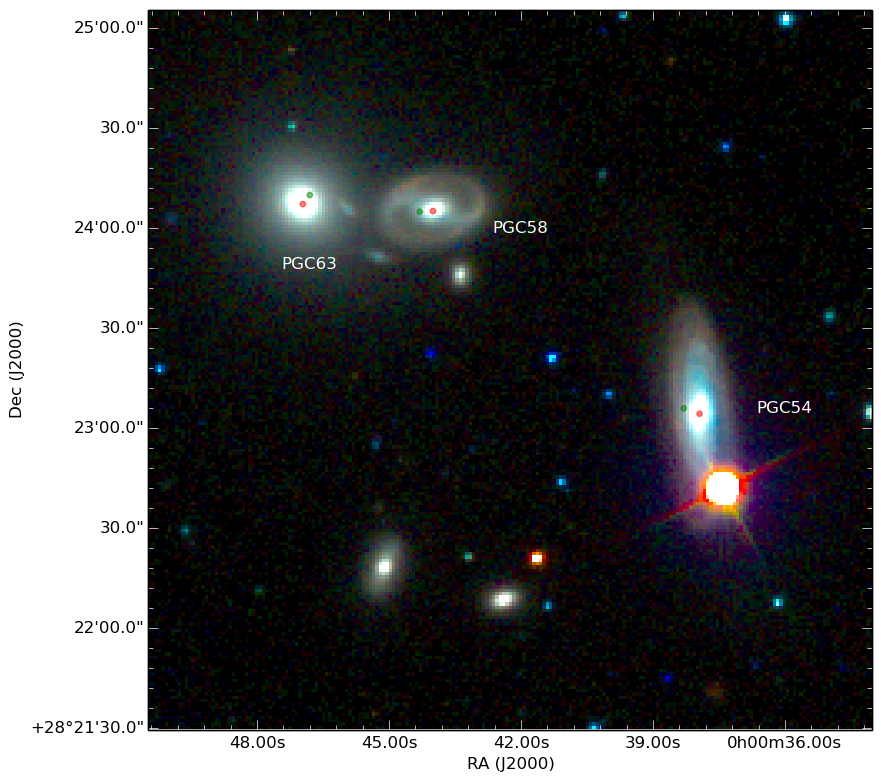
\includegraphics[width=0.5\textwidth]{figures/navigator}
		\caption{3 source confused RC3 Galaxies; Green marker denotes coordinates denoted in the RC3 catalog, red marker denotes coordinates updated by the algorithm}
	\end{figure}

%	\begin{figure}[h]
%
%		\begin{subfigure}{.5\textwidth}		
%		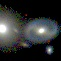
\includegraphics{figures/PGC58b4SC}		
%		\end{subfigure}		
%
%		\begin{subfigure}{.5\textwidth}		
%		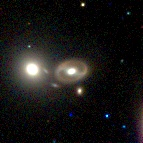
\includegraphics{figures/PGC58afterSC}
%		\end{subfigure}		
%
%	\end{figure}
\begin{figure}
\begin{subfigure}{.3\textwidth}
\centering
  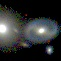
\includegraphics[width=.4\linewidth]{figures/PGC58b4SC}
  \caption{Before}
\end{subfigure}%
\begin{subfigure}{.3\textwidth}
\centering
  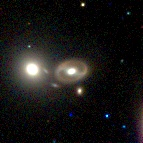
\includegraphics[width=.4\linewidth]{figures/PGC58afterSC}
  \caption{After}
\end{subfigure}
\caption{Using source confusion algorithm to generate mosaic centered at PGC58}
\label{fig:SCdemo}
\end{figure}
	%(One line intro about galaxies living close to each other==> galaxy cluster,gravity stuff?)
\indent Large galaxies tends to form gravitationally bound structure known as galaxy clusters . The source confusion algorithm works on the assumption that the only galaxies that are large enough to cause source confusion also lie in the RC3 catalog, since the catalog is reasonably complete for galaxies having apparent diameters larger than 1 arcmin. First, the program retrieves a list of n number of RC3 galaxies that may lie in the field of view of the generated mosaic. The $\texttt{otherRC3}$ method in the $\texttt{Server}$ class queries this information using the Vizier Catalog. If this information is provided by a survey's query service (such as the RC3 Table in SDSS's SkyServer), it can be overridden. The goal is to match the results returned by the server with the list of n largest sources detected by SExtractor. 
\\
\indent  We need to cross-correlate the coordinate by matching together the relative differences between the sources, due to the unreliability of absolute coordinates inherent to the catalog as discussed in section 2.1. We assume that the positional inaccuracy is due to  instrumentation and measurement error but retains the galaxies' relative locations.  %no distortion that changes the relative positions among neighboring sources. 
Therefore, we compute all the possible distances between any two RC3 galaxies that lies in our field. Then compare this with the set of differences generated by the SExtractor-generated list. We select n number of galaxies that has the closest values in both list, thereby matching together the galaxies from the catalog  with the detected sources. Finally, we mosaic using that galaxy's coordinates as center. Our premises proves to be valid, as the algorithm executed with a success rate of 99.97\% in the SDSS run, and is capable of correctly resolving up to 8 RC3 sources in one example.
	%Some parts of the program needs to be adjusted for survey-specific , but the core concept (and bulk of the code) should stay the same. 
	%Think of a name to refer to "the program"
\section{Pipeline}
%We incorporate our automated mosaic-making framework to a general pipeline
%we designed a mosaicing pipeline that creates scientifically-calibrated mosaics, color-band images, as well as a set of updated positions, which can be easily adapted for existing surveys such as Two Micron All Sky Survey  (2MASS),The Palomar Digital Sky Survey (DPOSS), or future imaging data release from  Dark E
%We desgined a mosaicking pipeline that can 
	\subsection{Class Hierarchy}
	\begin{figure}[h]
		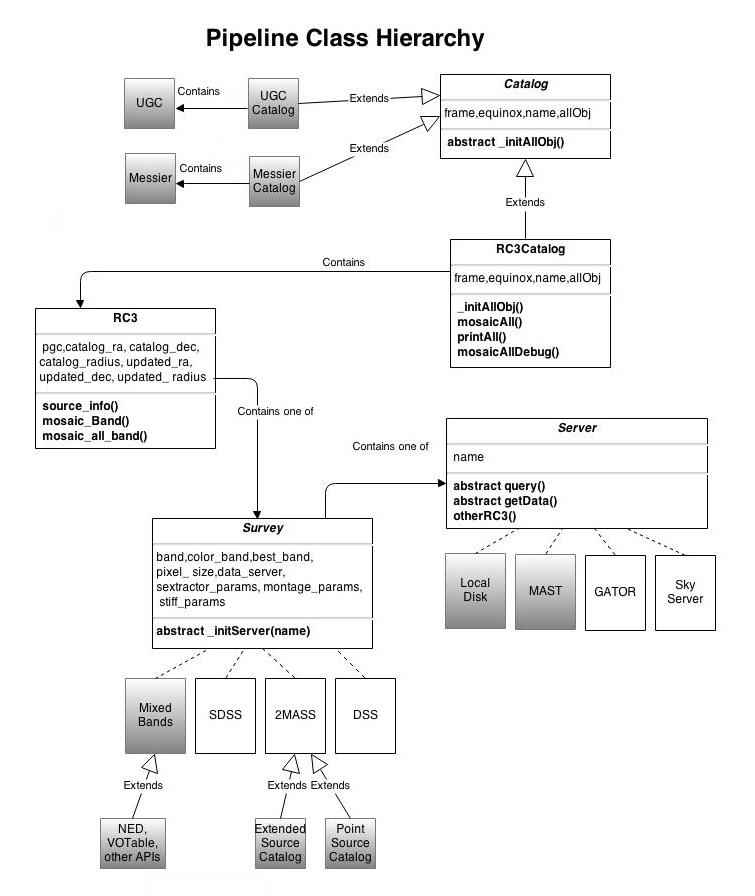
\includegraphics[width=0.5\textwidth]{figures/pipeline.jpg}
		\caption{Greyed out boxes are possible extensions of this pipeline}
	\end{figure}
 	The motivation behind building a class hierarchy is to establish a mosaicking pipeline for any given catalog and survey data. We identify the essential components required for mosaicking program to work. The relationship between these essential steps are reflected in our design of the abstract $\texttt{Survey}$,$\texttt{Catalog}$, and $\texttt{Server}$ classes. 
 		\paragraph{Server}
		Data acquisition is composed of two main tasks: querying imaging data and retrieving data from server. Most surveys have an API that enables data access by SQL or customized query. To make the $\texttt{Server}$ class work, we need to figure out how to convert positional values (ra,dec) to record-keeping parameters dependent on the survey's telescope. (e.g. tiles, frames...etc) For example, SDSS image frames are uniquely identified by a particular combination of  run, camcol, and field.  This step can usually be done using the SQL search. Our choice of using a server instead of a data object enables code reusability across various surveys that uses common server tools , such as IPAC's GATOR query service (\citet{irsa}) or  Astroquery.
	\paragraph{Catalog Objects}
	For the purpose of mosaicing RC3 galaxies, we did not create a $\texttt{CatalogObject}$ class, although it would be helpful to have a generic class similar to the functions in $\texttt{RC3Objects}$	. They perform the essential mosaicking features on a per-object basis so that they can be further used in the $\texttt{Catalog}$ class. The final step in the mosaic procedure generates 2 TIFF color images as described in Section (ALGORITHMS).  When extending the pipeline to other surveys, investigators can adjust the STIFF parameters to better suit the telescope-specific imaging details following the guidelines in \citet{stiff}.
	\paragraph{Catalog}
	The $\texttt{Catalog}$ class contains a list of objects that lies inside the catalog. Although the use of the Catalog container class seem unnecessary, it enables a clear separation between basic mosaicking functionality for individual galaxies. This can be used to study some particular object, executed on all objects in a $\texttt{Catalog}$, or simply used for debugging purposes. This abstraction barrier ensures minimal changes to the code in both classes when an investigator decides to input data from a new survey in the future.

		\subsection{Technical Details}
		Due to the recent surge in popularity of Python in astronomy, we wrote the program in Python 2.7.6 so that the program's dependencies are more widely supported for extending its usage on future datasets. Most of the mosaic steps are done using IPAC's Montage  \cite{montage} mosaic engine along with the AstroPy Montage wrapper\footnote{\url{http://www.astropy.org/montage-wrapper/}} and the final colored image is created using Astromatic's STIFF v.2.4 \cite{stiff}. Our choice of the two program makes use of the best features from both programs. Montage creates scientifically-calibrated images by retaining the astrometry and photometry of input sources during image reprojection step. STIFF provides the flexibility of adjusting many variables for the final colored image, as well as automatically estimating upper and lower cuts on the dynamic range using statistics derived from a pixel histogram.  %The use of two different program in the mosaicking step is due to Montage's ability to create scientifically-calibrated mosaic FITS, but STIFF provided more flexible parameters for combining all bands into color images, so we get the best of both worlds. 	The STIFF setting needs to be adjusted for each survey depending on specs on the telescope's CCD dependent parameters such as imaging bands and best quality bands.  
The source extraction is done using SExtractor v.2.19.5 (\citet{sextractor}). The resulting database was created using the Python sqlite3 module and the web search interface was written with PHP.

	\subsection{Known Errors}
	(Need to fix this section later ..)
	Even though a series of exception handling and error prevention mechanisms were put in place,  there are still errors in the data product that we produced.
	 	\begin{itemize}
	 		\item mProjectExec is the montage Mosaic procedure that creates the reprojected image from the raw FITS files. Sometimes reprojected images are not created even when Montages' debug statement clearly shows that the reprojection was successful and table and header files are corrupted. This results in an error in later mosaicing steps. We have implemented error prevention mechanism to ensure that mosaic procedures terminates correctly in such cases and wrote the problematic galaxy into failed\_projection, which can be examined later.
	 		\item Montage's background rectification module is not used in creating the FITS mosaics . Attempts were made in implementing these procedure, however it  is sometimes stuck in the step where the background model is applied to the projected images and  produces huge difference images files (\~50GB) for reason that we have not figured out yet. This should not affect the astrometric quality of the data product. The only visible diffference is observed in the color images for 2MASS, so will likely affect the photometric quality of the resulting 2MASS mosaics.(?)
	 	  \item (We should probably fix this?)There was more galaxies affected by the source confusion issue since we are only taking one photographic plate to crop, it doesn't actaully pass through the mosaicing algorithm. Subsequently,  it was never passed through the source confusion algorithm. 
	 	  %\item The Montage 	mBgExec takes a long time . 
	 		  %in coordir (\~)
	 	\end{itemize}
	
	\subsection{Performance}	
	\indent We accelerate the mosaicing process by performing the recursive algorithm on only a single band FITS file designated as $\texttt{best\_band}$, then mosacking all bands only once per object. For SDSS, we use the image obtained by the r band filter since transmission curve in \citet{edr} shows that r band has the highest quantum efficiency. 
	\\ \indent  Most of the computation time is spent on downloading the raw FITS files from the survey's specific server. Therefore, even though Montage's modular design enables its performance to scale with number of processor  (\citet{montage}), the process would not be significantly sped up by the use of Message Passing Interface (MPI). Therefore, the speed depends more on the bandwidth (downloading rate) rather than the number of cores in the machine. This average runtime would also depend on the sky coverage of the  particular survey and the speed of query.
	\\ \indent This process can  be significantly sped up if the investigator already has imaging data stored locally on a disk or have access to running the mosaic program alongside the survey's datacenter. We have designed our class hierarchy such that this can be written as a subclass of $\texttt{Server}$ with user-defined details of where the images are stored.


\subsection{Result from SDSS/DPOSS run}
\indent There are a total of 12512 RC3 galaxies within the SDSS footprint. The automated mosaicking pipeline was  successful for 90.22\% of the galaxies. 2446 RC3 galaxies is mosaiced using an updated position that was more than 1 arcminute off the values recorded in the RC3 catalog.  On ( bigdog specs)  machine, the program processes on average about 80 RC3 objects per hour using SDSS data.  %1.21 galaxies per minute, 
The finished data product occupies 31 GB of diskspace. 
\\
\indent  For the DPOSS Run, on average 0.31 galaxies per minute. (\#More on this later..)

 \section{Conclusion}
\indent Wide-area sky surveys are often used to answer fundamental questions regarding large-scale structure and the cosmological history of the universe. The mosaicking procedures described in this paper provides a convenient way to generate mosaics for sky survey imaging data for a given catalog, or on a per-image basis. This is easily adapted for future data to create the scientifically-calibrated FITS mosaics as well as colored images. 
\\
\indent Feeding in the new data enables a greater  sky coverage and higher resolution images of objects inside the catalog. The scientifically calibrated FITS images can be used as for individual studies, as well as used for improved astrometry in updating the catalog. It can also be combined with the calibrated mosaics of different wavelengths into multiband color images with mosaics from single/double band surveys such as POSS-I and GALEX.  %Can also do photometry to determine galaxy property 
%Another possible usage is to
\\
\indent The data product may also be useful  during  the target selection/commissioning stage of new sky survey programmes such as the LSST. With the trend of future telescope having larger aperture(focal plane?), large nearby galaxies needs to be properly masked to prevent the loss of imaging details from saturated CCDs. The updated RC3 coordinates tells us  which regions of the sky may be affected by these large galaxies, and the FITS files can be used for model-fitting the galaxy's light distribution. The FITS images can be used along with existing tools for scientific analysis, such as Astrometry.net(\citet{astrometry.net}) , SExtractor, APLpy(\citet{aplpy}). The program is designed such that other API with Programs interface such as HEASARC's SkyView, NED ..etc can easily be latched on (REFERENCE Fig1). This can also be extended for other astronomical catalog such as the Messier Catalog or New General Catalog (NGC), as well as catalogs with user-defined selection limit. %user-defined catalogs used for (group, cluster,target??) studies. 
%Can be incorporated in the photo pipeline in future survey to make pretty rc3 images.
%especially with the DSS data, full coverage of the sky
%map out where bright objects are. 
\\
\indent We have provided documentation on GitHub  that guides investigators through the steps to adapting the pipeline for future imaging data.The source code and documentation for the pipeline described in this paper can be found in the project repository: \url{https://github.com/ProfessorBrunner/rc3-sdss}. The data product from the SDSS and DPOSS run is available via a search form at \url{http://lcdm.astro.illinois.edu/search.html}.

\section*{Acknowledgements}
\footnotesize
\indent (Google\/ GSoC?) We thank Harold G. Corwin, Jr. for helpful discussion that helped this work. This research made use of Montage, funded by the National Aeronautics and Space Administration's Earth Science Technology Office, Computation Technologies Project, under Cooperative Agreement Number NCC5-626 between NASA and the California Institute of Technology. Montage is maintained by the NASA/IPAC Infrared Science Archive. This research made use of Astropy, a community-developed core Python package for Astronomy (Astropy Collaboration, 2013).
\\
\indent  Funding for SDSS-III has been provided by the Alfred P. Sloan Foundation, the Participating Institutions, the National Science Foundation, and the U.S. Department of Energy Office of Science. The SDSS-III web site is http://www.sdss3.org/. SDSS-III is managed by the Astrophysical Research Consortium for the Participating Institutions of the SDSS-III Collaboration including the University of Arizona, the Brazilian Participation Group, Brookhaven National Laboratory, University of Cambridge, Carnegie Mellon University, University of Florida, the French Participation Group, the German Participation Group, Harvard University, the Instituto de Astrofisica de Canarias, the Michigan State/Notre Dame/JINA Participation Group, Johns Hopkins University, Lawrence Berkeley National Laboratory, Max Planck Institute for Astrophysics, Max Planck Institute for Extraterrestrial Physics, New Mexico State University, New York University, Ohio State University, Pennsylvania State University, University of Portsmouth, Princeton University, the Spanish Participation Group, University of Tokyo, University of Utah, Vanderbilt University, University of Virginia, University of Washington, and Yale University

\bibliography{bibtex_database}
 \bibliographystyle{abbrvnat}
\end{document}
